\section{ICPR}

Al inicio se realizó una búsqueda de bases de datos que tuvieran diferentes rostros posicionados en distintos ángulos. Sin embargo, hubo una única base de datos pública publicada por la \textit{ICPR} \textit{(International Workshop on Visual Observation of Deictic Gestures)}, en Cambridge, Reino Unido, con  2790 imágenes disponibles para cualquier propósito. En esta base de datos cuenta con 15 sujetos de prueba, a cada sujeto se le realizaron dos pruebas y en cada prueba se realizó un total de 93 fotografías. El grupo de imágenes se obtuvieron al mezclar los siguientes ángulos: 7 de inclinación (vertical) y 13 panorámicos (horizontal) además de una dos fotografías extra, una en la posición completamente hacia arriba y otra completamente hacia abajo. Las imágenes en esta base de datos se encuentran en un formato JPG, además cada imagen cuenta con un documento de texto que contiene: el nombre del archivo y el centro en el eje X, en el eje Y, el alto y el ancho de la cara correspondiente. \cite{Gourier_Hall_Crowley}

Las fotografías de la base de datos se encuentran nombradas en primer lugar por su ángulo de panorámica y luego por su ángulo de inclinación, por lo que se puede observar que para cada sujeto las fotografías aparecen desde la panorámica extrema derecha y la inclinación extrema inferior y terminan en los extremos opuestos. Por lo que la fotografías recorren primero los ángulos de panorámica y luego incrementan los ángulos de inclinación. Además, estas fotografías no cuentan con algún archivo de etiquetas, por lo que estas se asignaron manualmente, tomando en cuenta el orden previamente explicado en que se encuentran ordenadas. A continuación se muestra un ejemplo del orden mencionado anteriormente:

\begin{figure}[H]
	\centering
	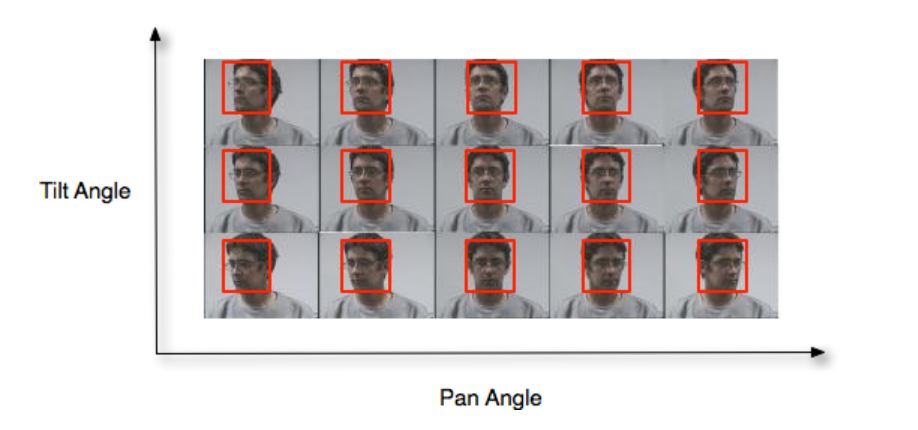
\includegraphics[scale=1]{figures/tiltpan.png}
	\caption{Muestra de 15 fotografías del sujeto 12 \cite{Gourier_Hall_Crowley}}
	\label{fig:img1}
\end{figure}

\begin{figure}[H]
	\centering
	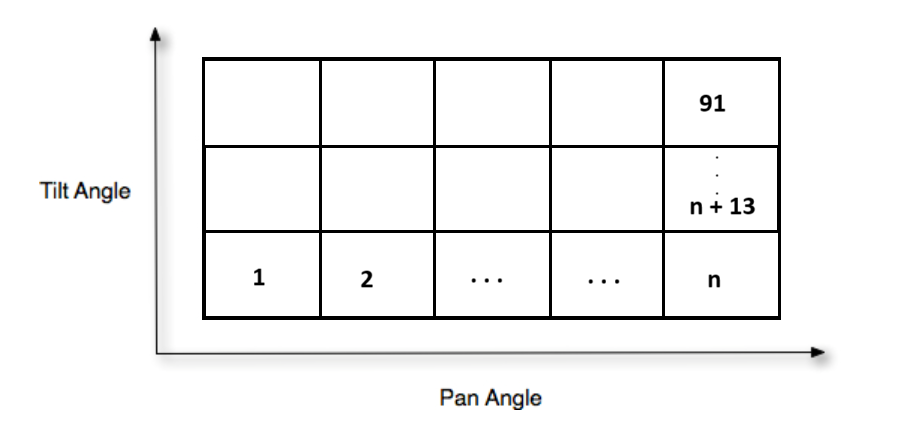
\includegraphics[scale=1]{figures/faceorder.png}
	\caption{Orden de guardado para cada serie de fotografías}
	\label{fig:img2}
\end{figure}

Además de este orden, todas las series de fotografías iniciaban con la imagen de la cabeza completamente hacia arriba y finalizaban con la posición completamente abajo, de frente para ambas. Dado que se tenían 15 sujetos de prueba, se procedió a guardar los archivos JPG de 11 (2046 imágenes) sujetos en un directorio de entrenamiento y los 4 (744 imágenes) restantes en el de pruebas. Al tener en cuenta el orden de los archivos y la cantidad en cada directorio se procedió a realizar las etiquetas por medio de un documento \textit{Excel}con formato \textit{.xlsx}. En dicho documento se creó una hoja para cada grupo de etiquetas, esto quiere decir, una hoja para etiquetas de entrenamiento y otra para etiquetas de prueba. Por lo que, en cada hoja se puede encontrar una columna con las etiquetas en el orden establecido en la Figura 2.

\subsection{Etiquetas para clasificación}

Para la primera experimentación se consideró clasificar las imágenes en 9 clases diferentes, de tal manera que la orientación de la cabeza respecto de la cámara funcionara de manera similar a una palanca de mandos analógica. A continuación se presenta una visualización de dicha clasificación:

\begin{figure}[H]
	\centering
	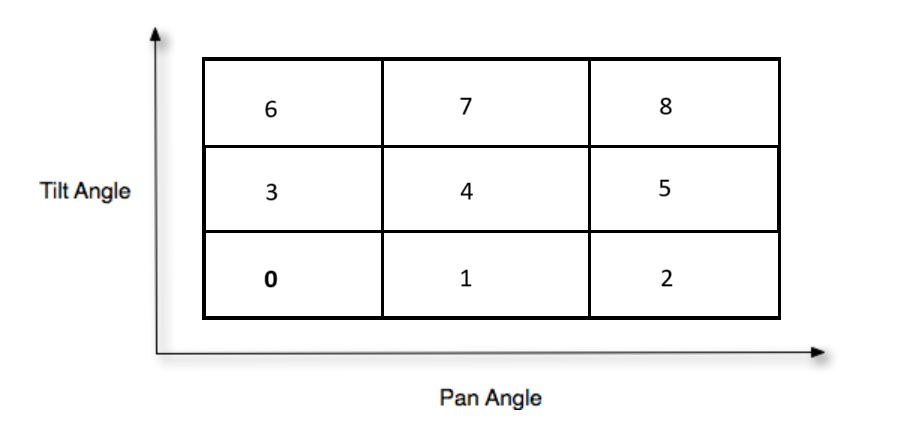
\includegraphics[scale=1]{figures/clasi0.png}
	\caption{Clasificación de imágenes en 9 etiquetas}
	\label{fig:img3}
\end{figure}

Utilizando esta cantidad de clases, se realizaron dos formas de etiquetado en las imágenes, en las cuales solo varía la cantidad de fotografías que fueron etiquetadas dentro de una clase u otra. En las siguientes figuras se podrá observar que la dimensión de cada celda está representada con (n $\times$ m), dónde n corresponde a la cantidad de ángulos panorámicos que abarca y m la cantidad de ángulos de inclinación (según las muestras tomadas del ICPR). Además, la posición de las celdas en las gráficas si corresponde a la numeración de la Figura 2.


\begin{figure}[H]
	\centering
	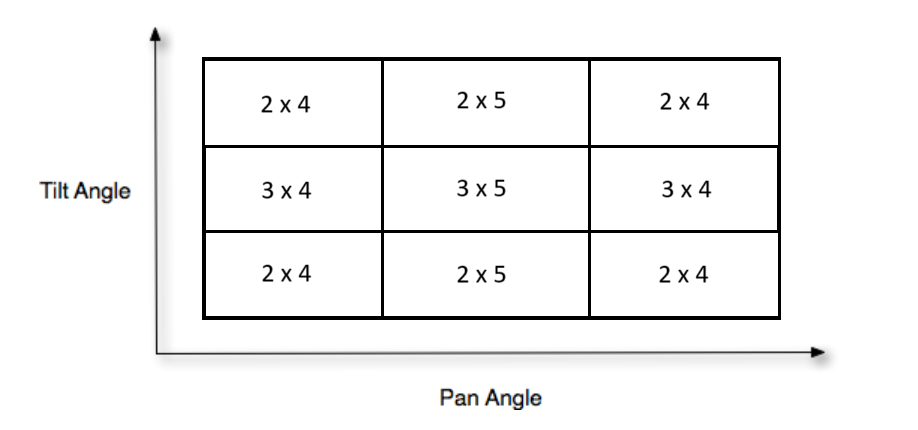
\includegraphics[scale=1]{figures/clasi01.png}
	\caption{Primera distribución de etiquetas}
	\label{fig:img4}
\end{figure}

\begin{figure}[H]
	\centering
	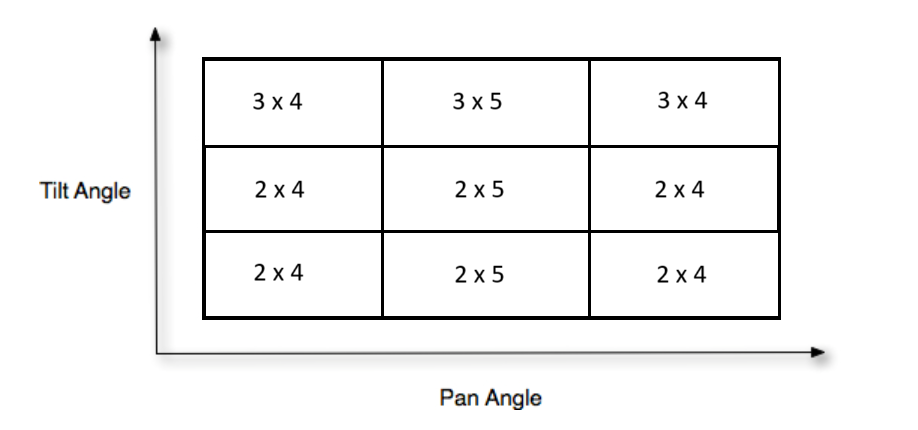
\includegraphics[scale=1]{figures/clasi02.png}
	\caption{Segunda distribución de etiquetas}
	\label{fig:img5}
\end{figure}

Luego de pruebas realizadas con resultados no satisfactorios en la sección de algoritmos para visión por computadora, la siguiente experimentación consistió en reducir la cantidad de clases a 6. En este caso para realizar un movimiento hacia atrás, se requiere un giro completo, en vez del sistema de joystick propuesto anteriormente. La división de clases se muestra a continuación:

\begin{figure}[H]
	\centering
	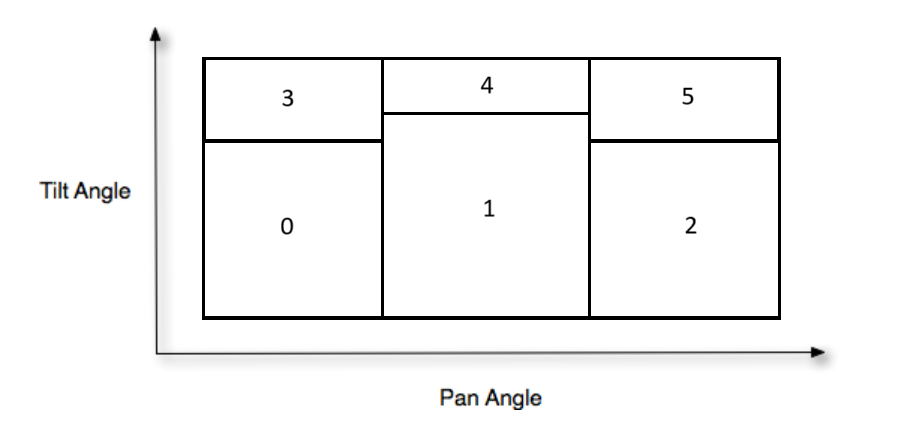
\includegraphics[scale=1]{figures/clasi1.png}
	\caption{Clasificación de imágenes en 6 etiquetas}
	\label{fig:img6}
\end{figure}

\begin{figure}[H]
	\centering
	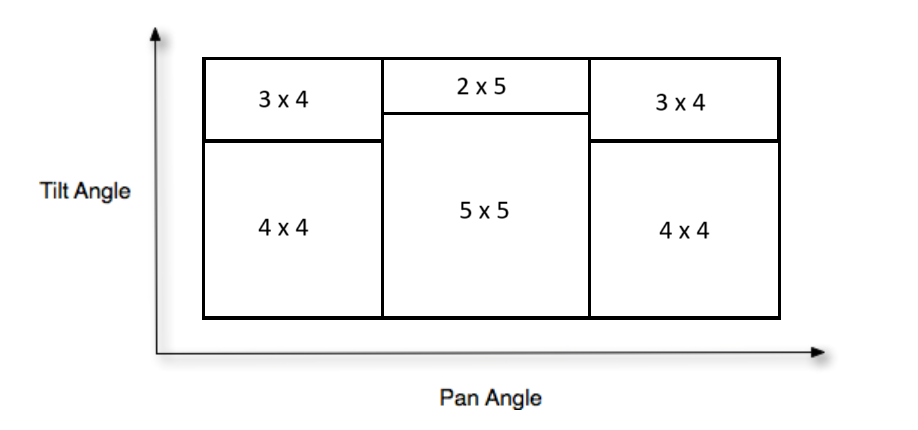
\includegraphics[scale=1]{figures/clasi2.png}
	\caption{Tercera distribución de etiquetas}
	\label{fig:img7}
\end{figure}

\begin{figure}[H]
	\centering
	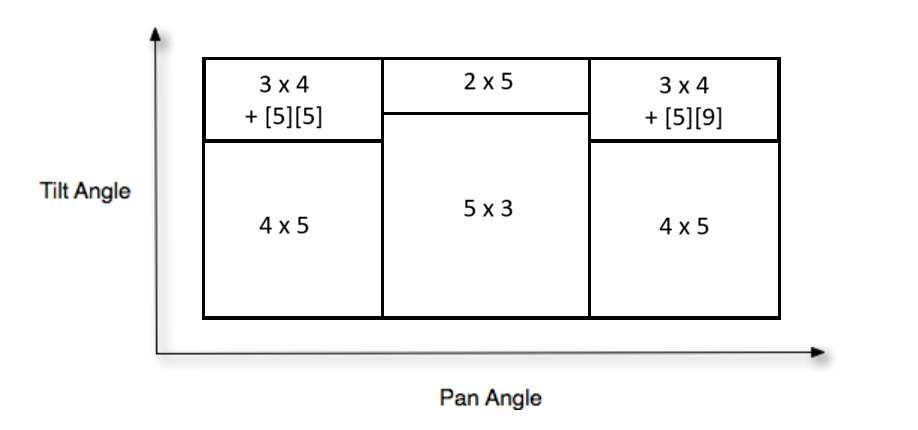
\includegraphics[scale=1]{figures/clasi3.png}
	\caption{Cuarta distribución de etiquetas (Las posiciones se cuentan desde la esquina inferior izquierda)}
	\label{fig:img8}
\end{figure}

\subsection{Etiquetas parte 2}
En esta ocasión se cuenta con 4 series nuevas de fotografías del usuario, en este caso Gerardo Fuentes (autor), que se agregan al set de entrenamiento, sin embargo, también se requerirá realizar una disminución de clases nuevamente. La nueva cantidad para la primera es de 4, y se tomarán en cuenta la posición de la cabeza en estado neutro, a los lados y hacia arriba o abajo. Luego de obtener el resultado, se realizará una nueva prueba de etiquetas con únicamente 3 clases, al centro y a los lados. 


\subsection{Fotografías personales}
Dado que los resultados con los modelos de de reconocimiento de orientación no fueron los esperados en ningún caso, se procedió a realizar 2 series de fotografías personales con la cámara integrada. Cada serie consta de 9 fotografías con posiciones que simulan las 9 clases inicialmente definidas a una distancia de 45 cm aproximadamente. Las series fueron capturadas en un salón de laboratorio del Departamento de Ingeniería Electrónica, Mecatrónica y Biomédica de la Universidad del Valle de Guatemala y en espacio diversos en la casa de Gerardo Andres Fuentes Bámaca (autor). Luego, las fotografías fueron renombradas de tal manera que se pudiera conocer su orden y posición en la lista de imágenes del grupo de entrenamiento. De esta manera, fueron agregadas las etiquetas correspondientes en el documento de etiquetas con extensión \textit{.xlsx}, tanto para los casos de 9 y 6 clases.

\subsection{Fotografías personales parte 2}
En esta ocasión, realizaron dos nuevas series de fotografías en casa de Gerardo Fuentes (autor), con las cuales se llega a un total de 4 series. Dado que las pruebas con el rostro del autor ser realizan con la actualización de cámara en tiempo real, las nuevas series de fotografías serán agregadas al set de entrenamiento. De esta manera, se generarán nuevos modelos de reconocimiento de orientación de cabeza. 



\section{ColorFET}